\chapter{Resultados y análisis}

Para cada uno de los experimentos con los autómatas celulares se utilizaron los siguientes parámetros:

\begin{itemize}
	\item \textbf{Vecindario:} de tipo Moore con 8 vecinos.
	\item \textbf{Parámetros de GA-Nuggets:}
	\begin{itemize}
		\item $w1=1$ 
		\item $w2=2$ 
		\item $\beta=2$ 
		\item $pMutacion=0.05$
		\item $noHijos=2$ 
		\item $poblacion=100$ 
		\item $noIteraciones=100$
		\item $maximoAntecedente=50$
		\item $minimoAntecedente=3$
	\end{itemize}
	\item \textbf{Parámetros de LRDEA:}
	\begin{itemize}
		\item $noHijos=2$
		\item $poblacion=100$
		\item $pMutacion=0.05$
		\item $noIteraciones=100$
	\end{itemize}
\end{itemize}

\section{Brain}

Como podemos ver en la figura \ref{fig:ra1brain} el algoritmo RA1 tuvo un muy buen desempeño con un promedio de exactitud de 89\% dentro del conjunto de datos y de 85\% en fuera del conjunto  a comparación del algoritmo LRDEA (figura \ref{fig:lrdeabrain}) que obtuvo un promedio de 88\% y 81\% respectivamente y el algoritmo GA-Nuggets con 88\% y 79\% (figura \ref{fig:ganuggetsabrain}).

	\begin{figure}[H]
		\centering
		\includegraphics[width=\linewidth]{fig/ra1_0}
		\caption{Exactitud de el algoritmo RA1 sobre el conjunto de datos del AC Brain.}
		\label{fig:ra1brain}
	\end{figure}

	\begin{figure}[H]
		\centering
		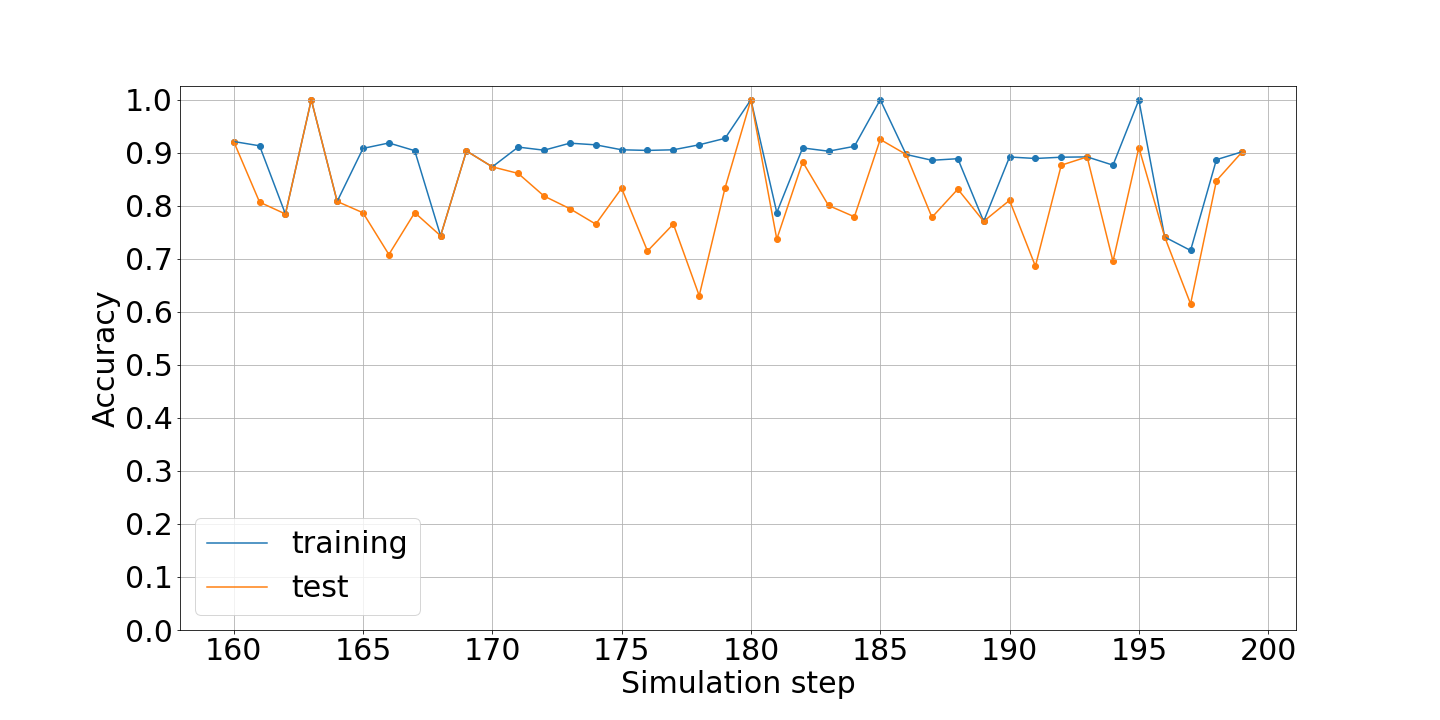
\includegraphics[width=\linewidth]{fig/LRDEA_1}
		\caption{Exactitud de el algoritmo LRDEA sobre el conjunto de datos del AC Brain.}
		\label{fig:lrdeabrain}
	\end{figure}

	\begin{figure}[H]
		\centering
		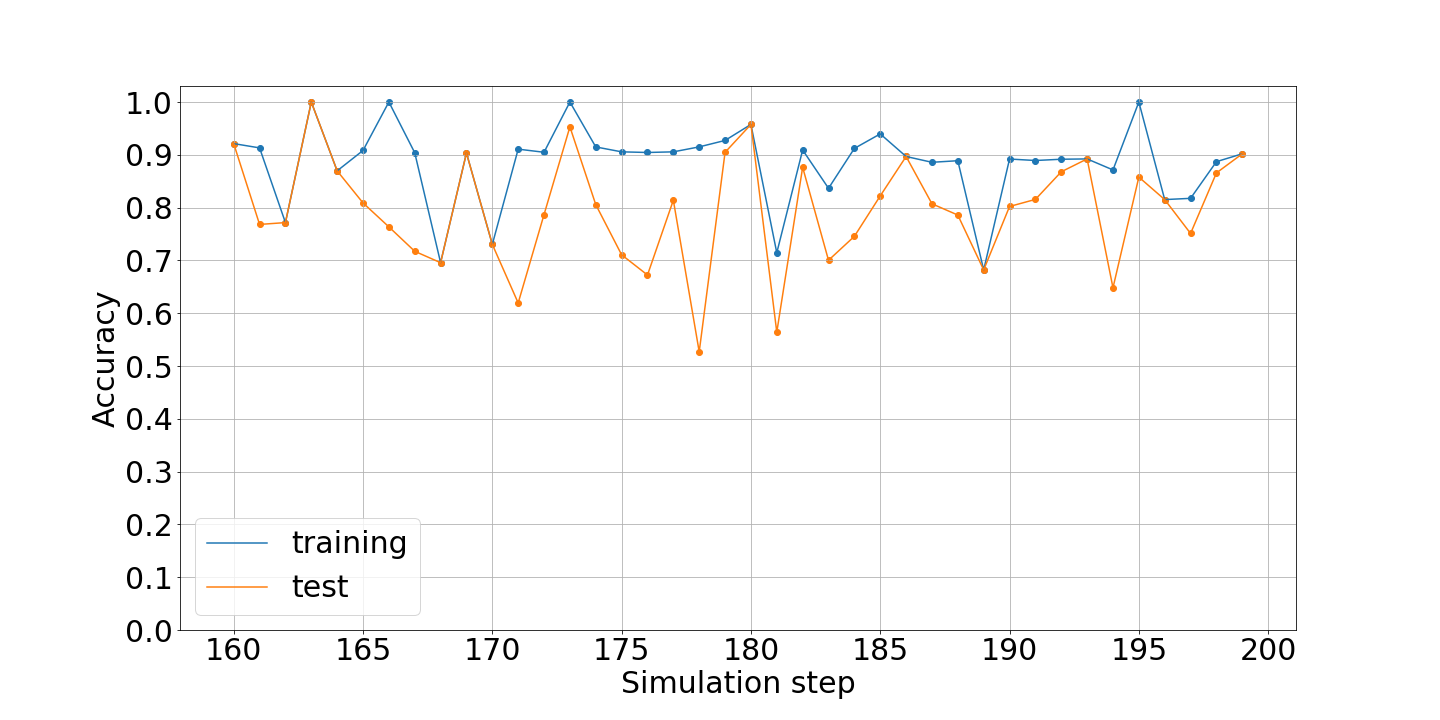
\includegraphics[width=\linewidth]{fig/GA-nuggets_2}
		\caption{Exactitud de el algoritmo GA-Nuggets sobre el conjunto de datos del AC Brain.}
		\label{fig:ganuggetsabrain}
	\end{figure}

\section{Byl}

Como se logra apreciar en ciertos estados se logro obtener una exactitud del 100\% esto es debido a que ciertos estados tienen un comportamiento mas trivial que los otros, lo cual resulta mas fácil de aprender para los algoritmos. De igual forma el algoritmo que obtuvo mejor valor de exactitud fue el RA1 con un promedio de 90\% en el conjunto de entrenamiento y un 85\% fuera del conjunto de entrenamiento, el algoritmo LRDEA obtuvo un promedio de 91\% y 84\% esto nos indica que el algoritmo tiene mas variación con respecto al RA1, y por ultimo el algoritmo GA-Nuggets obtuvo 89\% y 77\% con mayor variación y peor valor de exactitud con respecto a los otros dos algoritmos.
\begin{figure}[H]
	\centering
	\includegraphics[width=\linewidth]{fig/ra1_3}
	\caption{Exactitud de el algoritmo RA1 sobre el conjunto de datos del AC Byl.}
	\label{fig:ra1byl}
\end{figure}

Es interesante notar como en la figura \ref{fig:lrdeabyl} y la figura \ref{fig:ganuggetsabyl} se ve un comportamiento similar a comparación con la figura \ref{fig:ra1byl}, esto puede deberse a las dinámicas que rigen a los algoritmos genéticos, podríamos esperar que el algoritmo RA1 sea menos propenso a variaciones por que depende en menor medida de la probabilidad.
\begin{figure}[H]
	\centering
	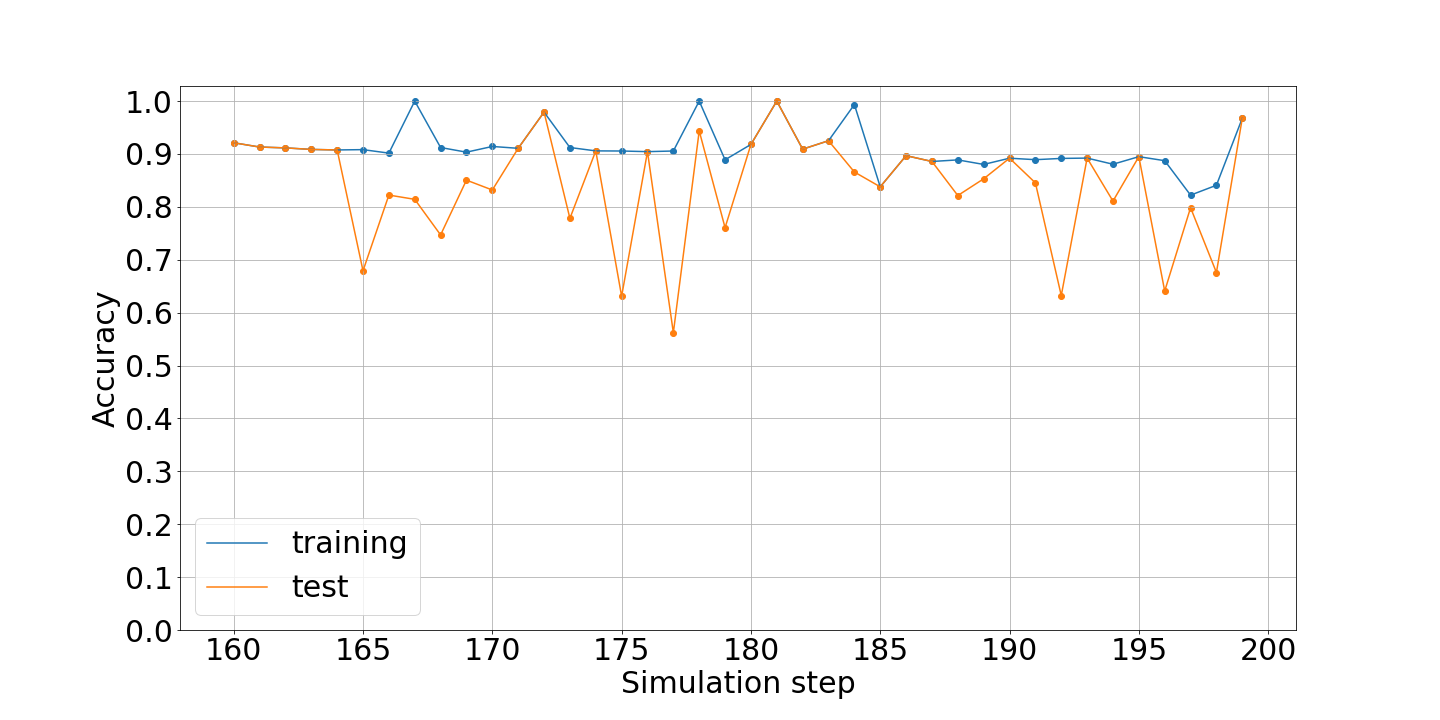
\includegraphics[width=\linewidth]{fig/LRDEA_4}
	\caption{Exactitud de el algoritmo LRDEA sobre el conjunto de datos del AC Byl.}
	\label{fig:lrdeabyl}
\end{figure}

\begin{figure}[H]
	\centering
	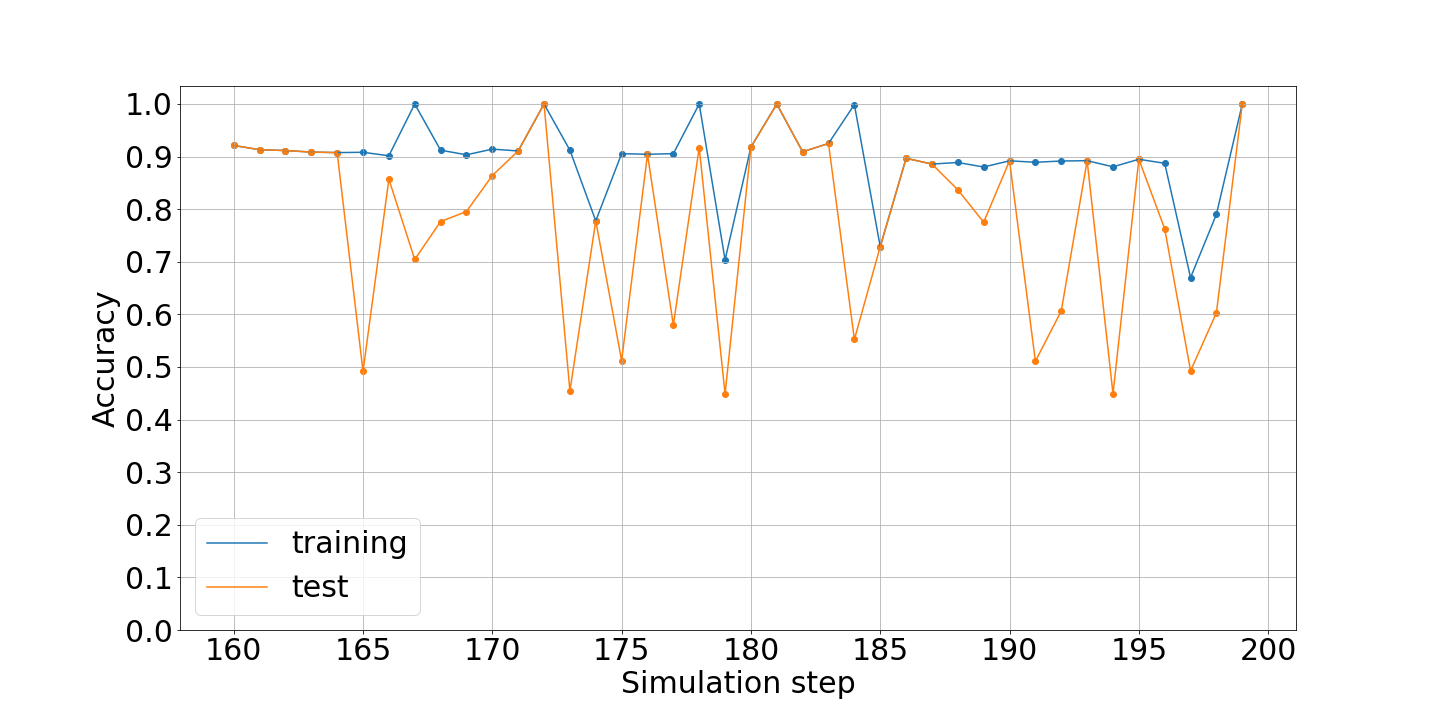
\includegraphics[width=\linewidth]{fig/GA-nuggets_5}
	\caption{Exactitud de el algoritmo GA-Nuggets sobre el conjunto de datos del AC Byl.}
	\label{fig:ganuggetsabyl}
\end{figure}

\section{Evoloops}
Al igual que con Byl este experimento fue uno de los que obtuvo mejor desempeño, con un promedio de 90\% de exactitud dentro del entrenamiento y 86\% fuera de entrenamiento el algoritmo RA1 fue el que obtuvo la mejor exactitud, en segundo lugar el algoritmo LRDEA con 89\% y 82\%, y por ultimo el algoritmo GA-Nuggets con 88\% y 78\%.
\begin{figure}[H]
	\centering
	\includegraphics[width=\linewidth]{fig/ra1_6}
	\caption{Exactitud de el algoritmo RA1 sobre el conjunto de datos del AC Evoloops.}
	\label{fig:ra1evoloops}
\end{figure}
\begin{figure}[H]
	\centering
	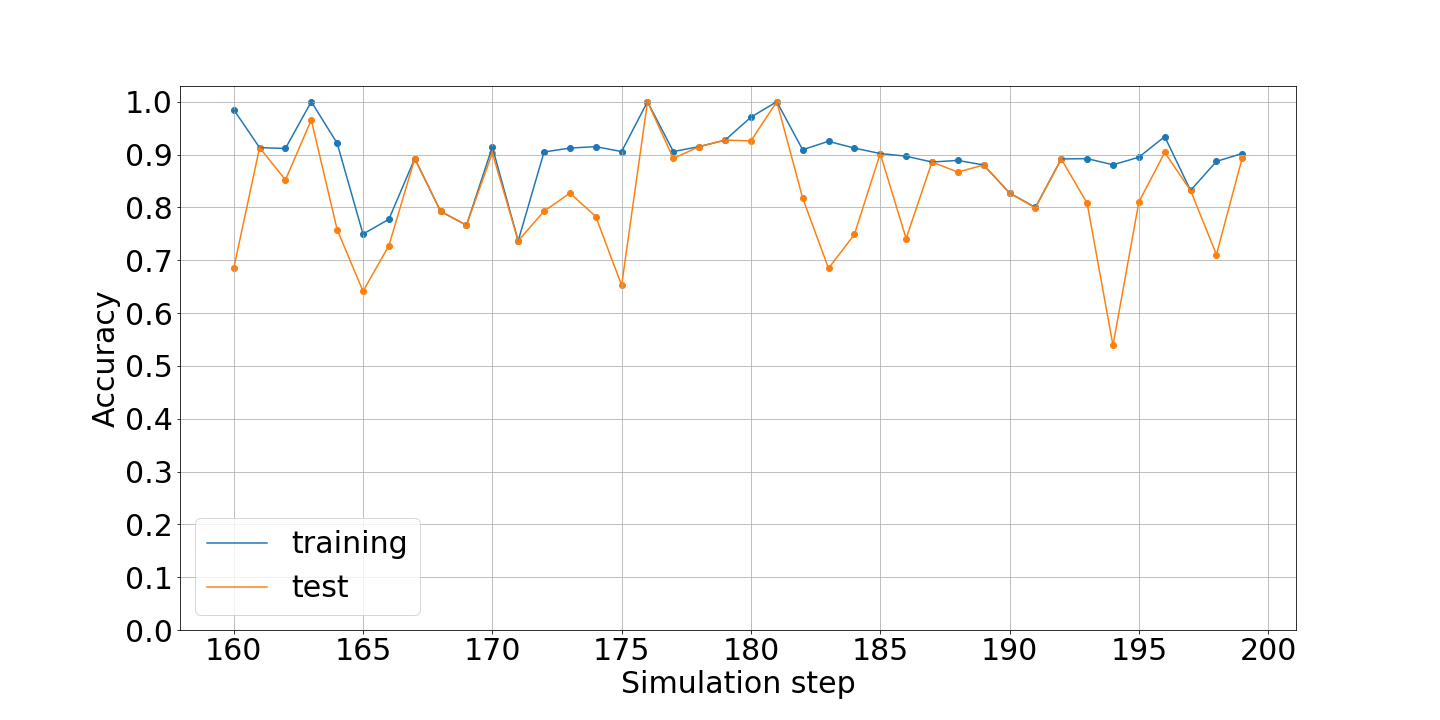
\includegraphics[width=\linewidth]{fig/LRDEA_7}
	\caption{Exactitud de el algoritmo LRDEA sobre el conjunto de datos del AC Evoloops.}
	\label{fig:lrdeaevoloops}
\end{figure}

En la siguiente gráfica podemos ver como el GA-Nuggets puede tener mucha variación en su exactitud, con respecto a los otros dos algoritmos.

\begin{figure}[H]
	\centering
	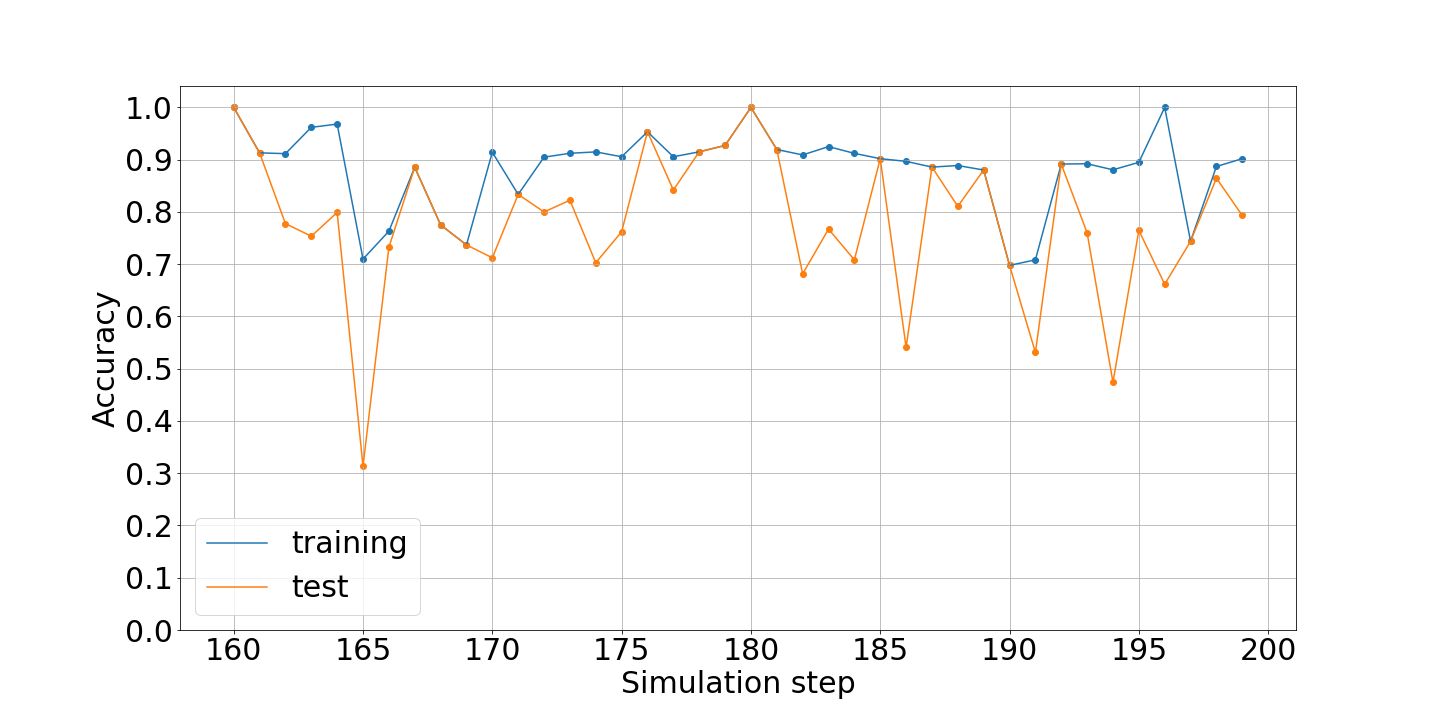
\includegraphics[width=\linewidth]{fig/GA-nuggets_8}
	\caption{Exactitud de el algoritmo GA-Nuggets sobre el conjunto de datos del AC Evoloops.}
	\label{fig:ganuggetsevoloops}
\end{figure}
\section{Mite}
Este experimento fue en el que se obtuvieron los resultados mas bajos, sin embargo, aun así logramos ver que nuestra propuesta sigue siendo capaz de mantenerse a un buen nivel en comparación a los otros dos algoritmos. Los promedios de exactitud dentro y fuera de entrenamiento son los siguientes: RA1 con 89\% y 84\%, LRDEA con 89\% y 81\%, y por ultimo GA-Nuggets con 88\% y 75\%.
\begin{figure}[H]
	\centering
	\includegraphics[width=\linewidth]{fig/ra1_9}
	\caption{Exactitud de el algoritmo RA1 sobre el conjunto de datos del AC Mite.}
	\label{fig:ra1mite}
\end{figure}
\begin{figure}[H]
	\centering
	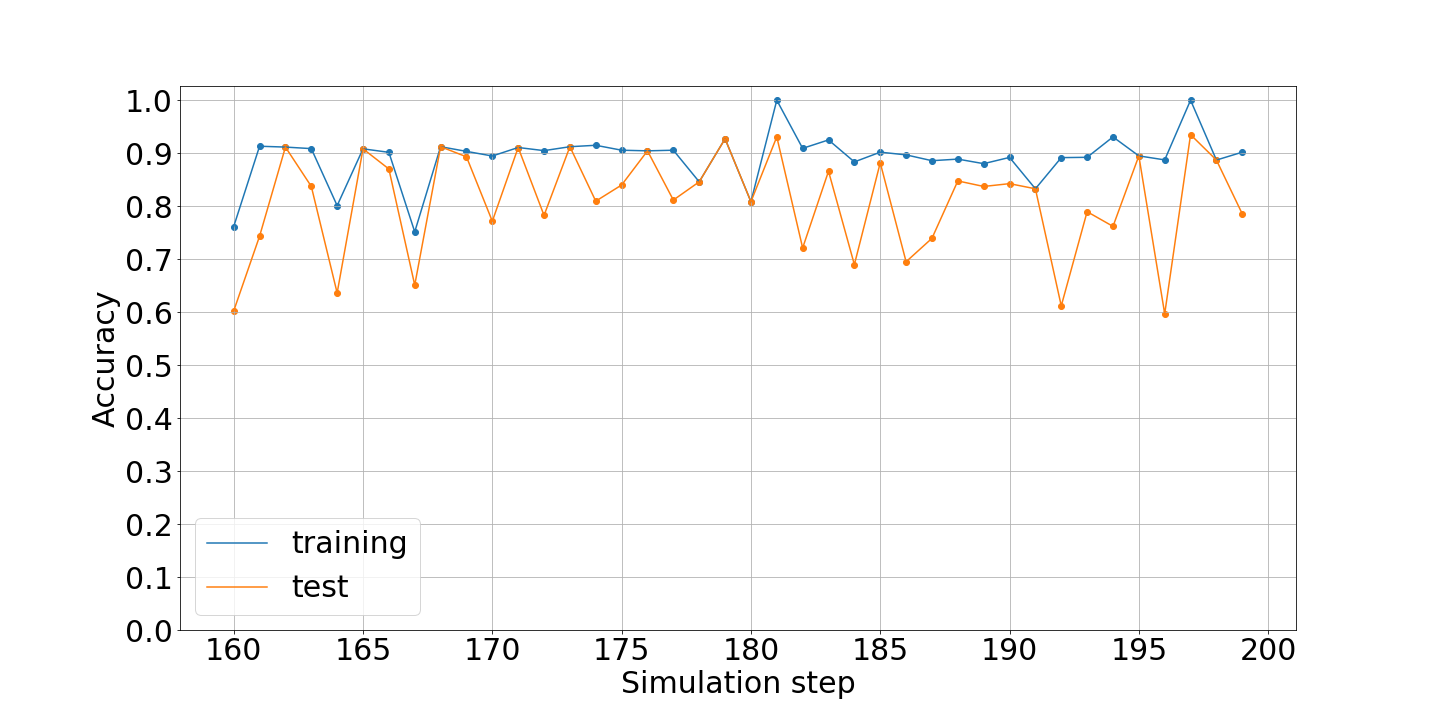
\includegraphics[width=\linewidth]{fig/LRDEA_10}
	\caption{Exactitud de el algoritmo LRDEA sobre el conjunto de datos del AC Mite.}
	\label{fig:lrdeamite}
\end{figure}

\begin{figure}[H]
	\centering
	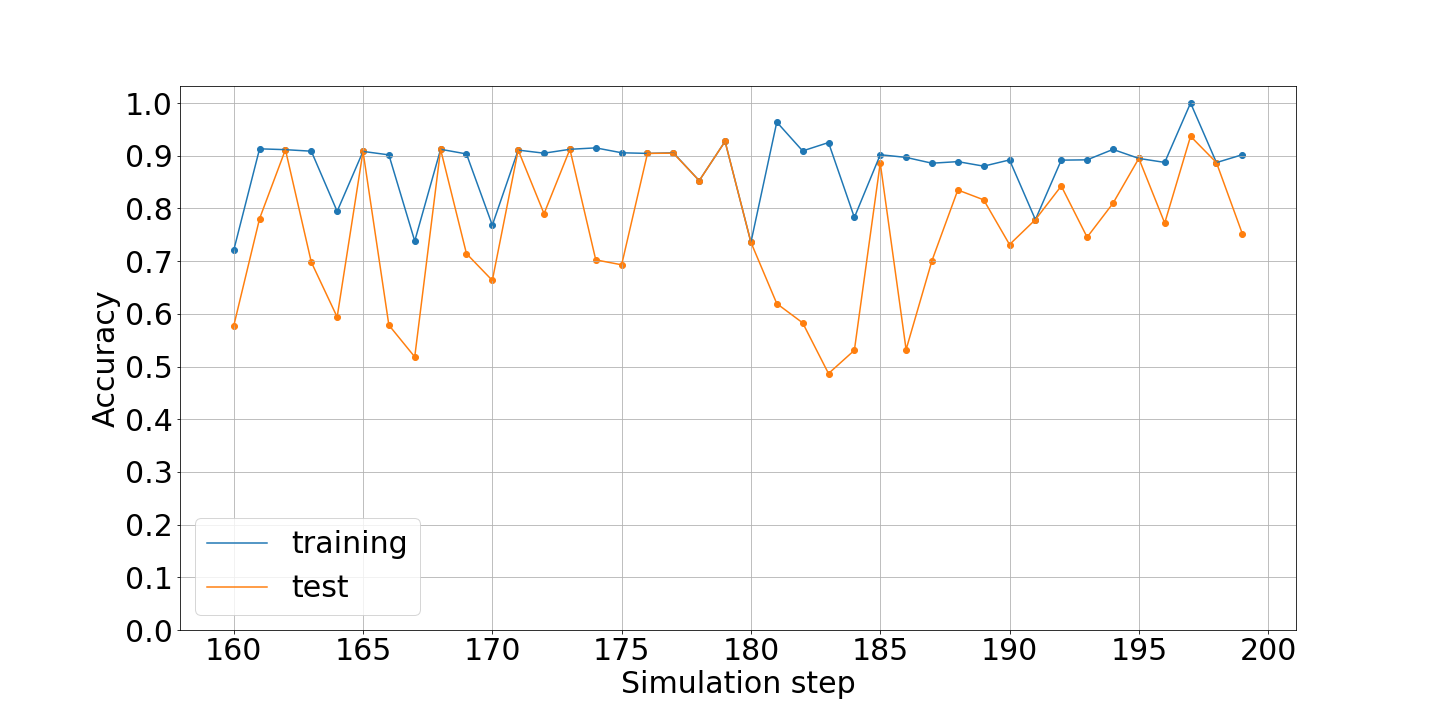
\includegraphics[width=\linewidth]{fig/GA-nuggets_11}
	\caption{Exactitud de el algoritmo GA-Nuggets sobre el conjunto de datos del AC Mite.}
	\label{fig:ganuggetsmite}
\end{figure}